% DO NOT COMPILE THIS FILE DIRECTLY!
% This is included by the other .tex files.

\begin{frame}[t,plain]
\titlepage
\end{frame}

\begin{frame}
  \frametitle{The aim of this presentation}
  \begin{itemize}
    \item Cerebrate
    \begin{itemize}
     \item What has happened since the last MUG
     \item Give you a brief update over the highlights
     \item Ongoing work
    \end{itemize}
  \end{itemize}
\end{frame}

\begin{frame}
  \frametitle{Statistics}
  \begin{itemize}
    \item Since the last MUG we've had:
    \begin{itemize}
        \item {\bf 4} releases
        \item {\bf 83} commits
    \end{itemize}
  \end{itemize}
\end{frame}

\begin{frame}
  \frametitle{CNW Pilot}
  \begin{itemize}
    \item Collaboration with ENISA and CNW community
    \begin{itemize}
        \item Bug fixes
        \item Usability rework
        \item Additional supporting tools
        \item New feature requests
        \item Security fixes
    \end{itemize}
  \end{itemize}
\end{frame}

\section{Give you a brief update over the highlights}


\begin{frame}
\frametitle{Enumerations}
    \begin{itemize}
        \item Create lists of enumerations for selector fields
        \item Unified way of expressing countries, types of organisations
        \item Created ad-hoc per instance
    \end{itemize}
    \begin{center}
        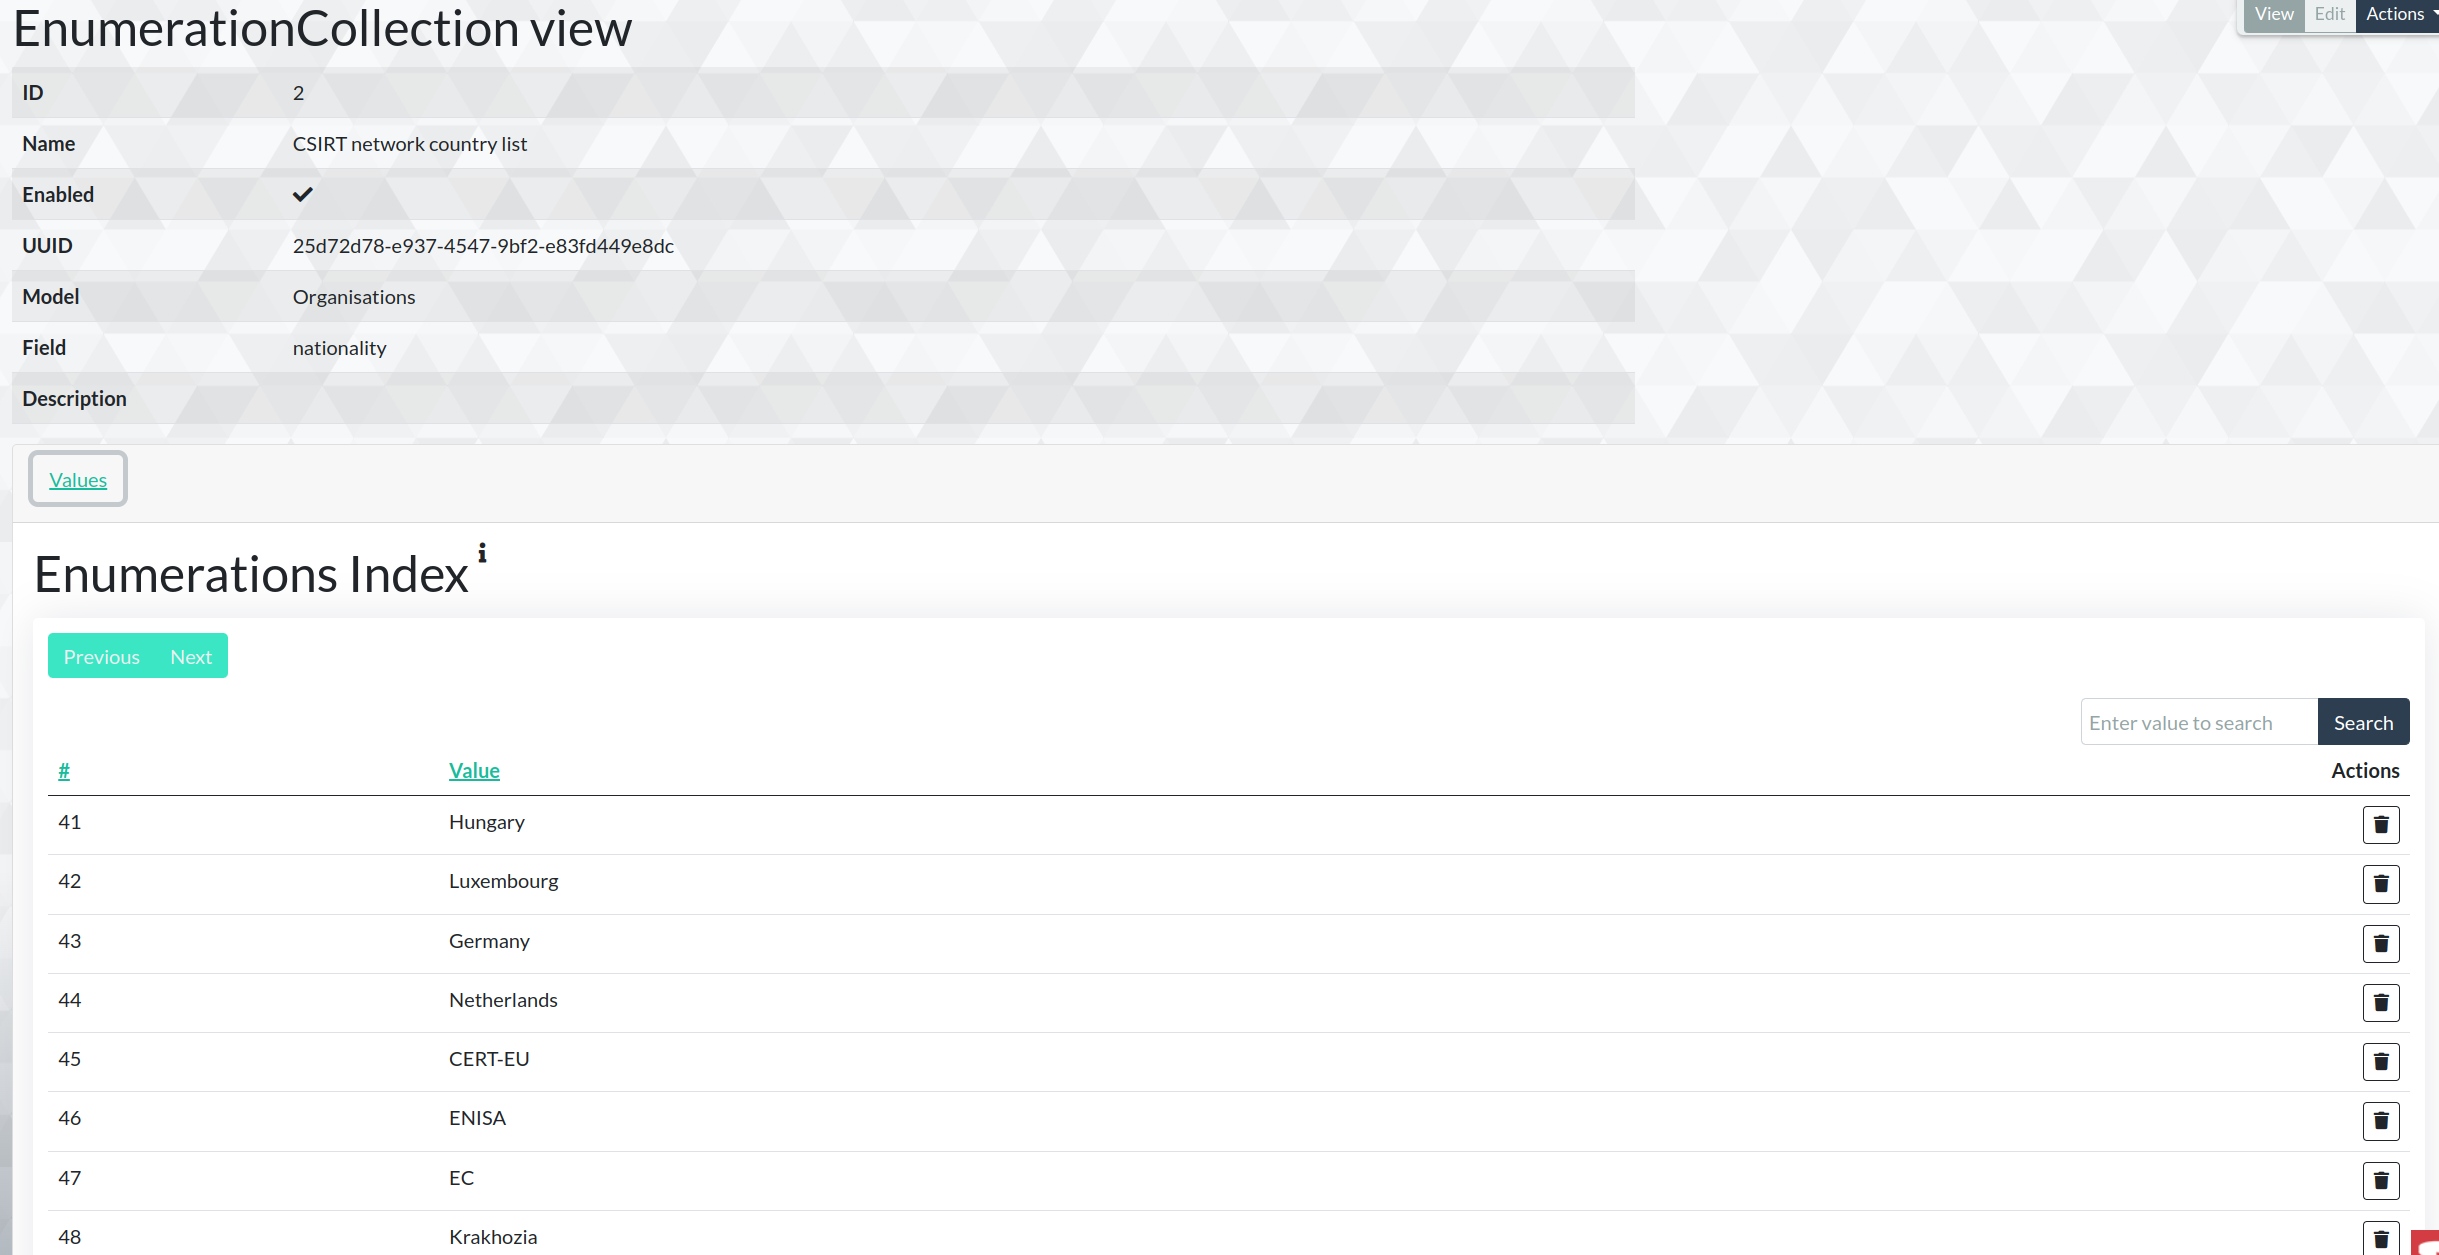
\includegraphics[width=1.0\linewidth]{pictures/enumeration.png}
    \end{center}
\end{frame}

\begin{frame}
\frametitle{Organisation group management}
    \begin{itemize}
        \item Create {\bf sub-groups} in the community
        \item For example national groups, with appointed administration
        \item Improve {\bf life-cycle management of user accounts}
    \end{itemize}
\end{frame}

\begin{frame}
\frametitle{Organisation group management}
    \begin{center}
        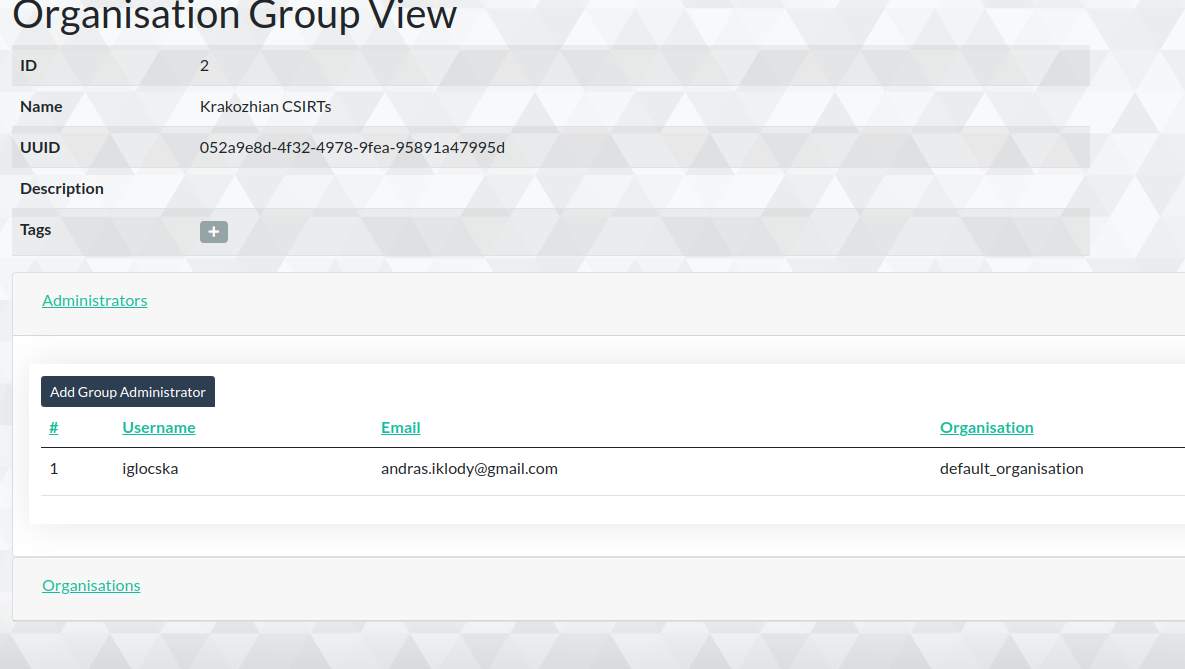
\includegraphics[width=1.0\linewidth]{pictures/OrgGroup.png}
    \end{center}
\end{frame}


\begin{frame}
\frametitle{MISP management}
    \begin{itemize}
        \item Be able to manage {\bf Cerebrate interconnections}...
        \item ...and {\bf MISP instances}
        \item Visual overview, simple access
        \item Debugging and diagnostics
        \item Data management
    \end{itemize}
\end{frame}

\begin{frame}
\frametitle{Topology}
    \begin{center}
        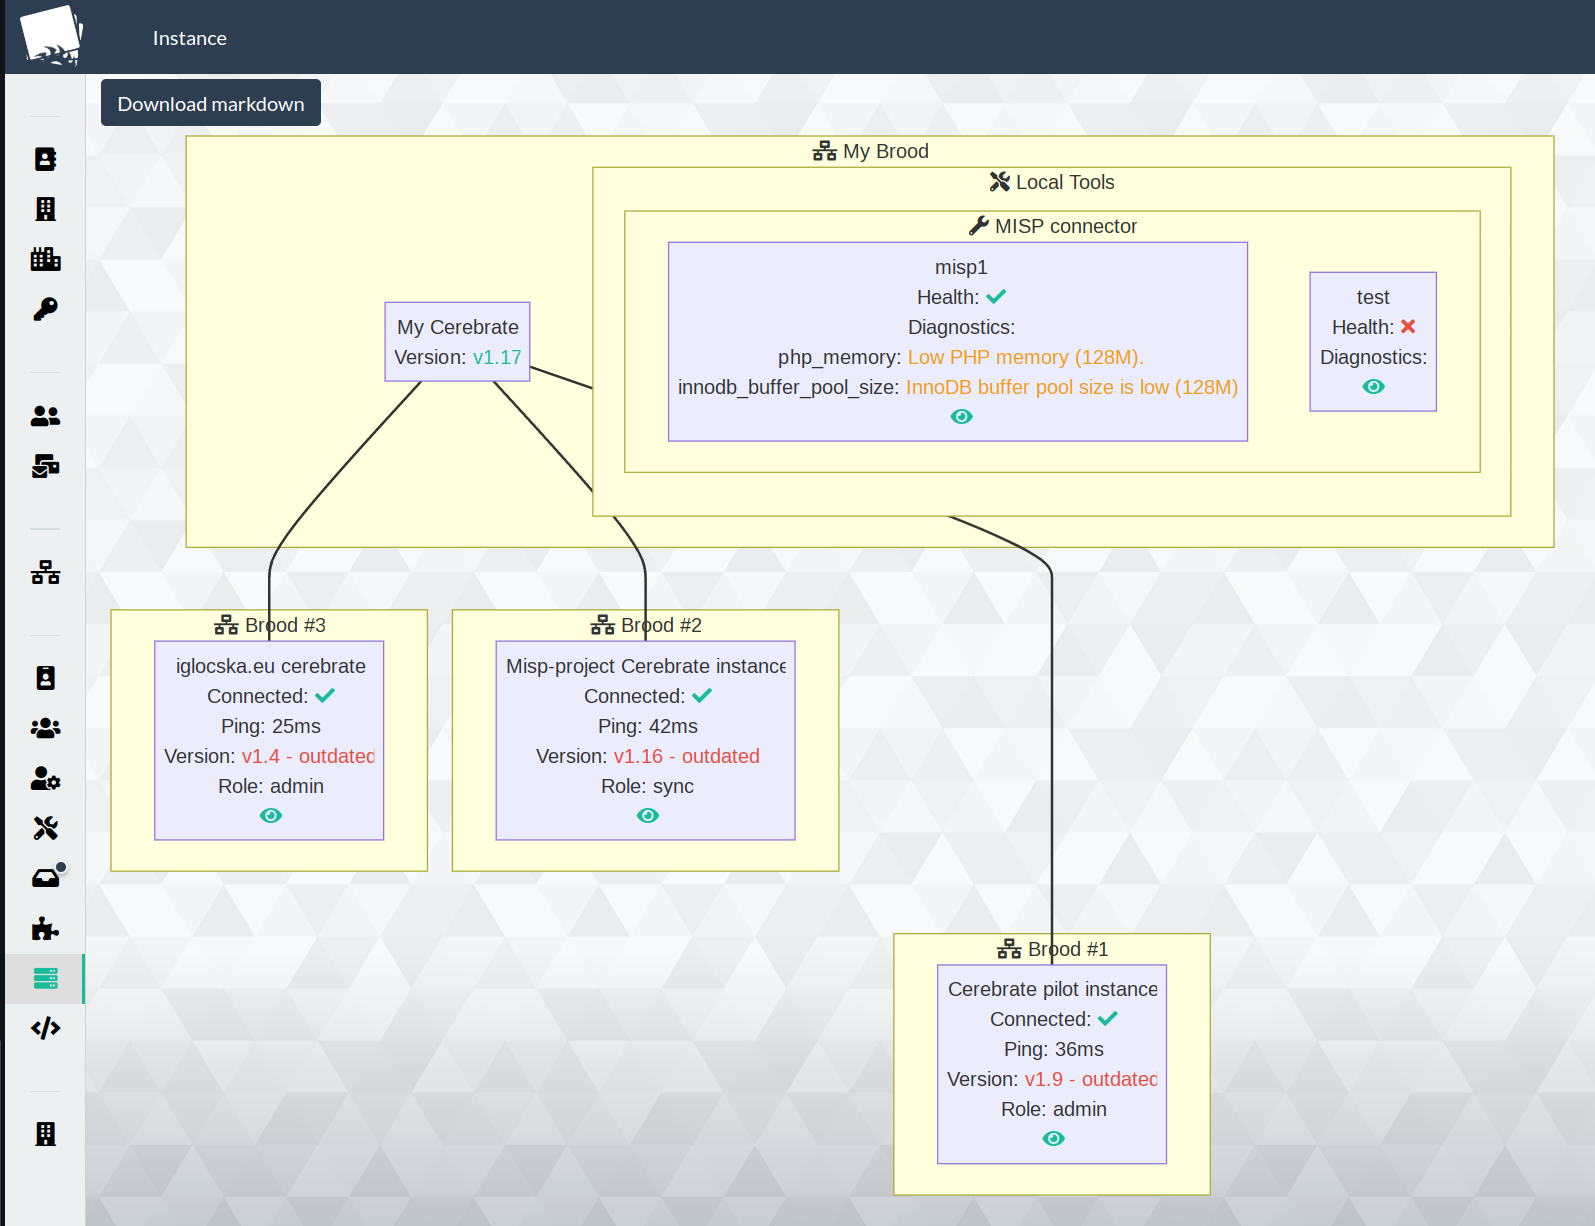
\includegraphics[width=1.0\linewidth]{pictures/orchestration1.png}
    \end{center}
\end{frame}

\begin{frame}
\frametitle{MISP management}
    \begin{itemize}
        \item Built using {\bf mermaid.js}
        \item Can export itself as mermaid markdown
        \item Easy to use for documentation
        \item {\bf Diagnostics} relies on connector module implementation
        \item Quick {\bf pivots} to all tool and connected cerebrate functinalities
    \end{itemize}
\end{frame}

\begin{frame}
\frametitle{MISP connector updates}
    \begin{itemize}
        \item New features to better negotiate information exchange
        \item View / compare {\bf state} of data repositories
        \item Multi-select {\bf bulk ingest}
        \item Rule based {\bf bulk push}
    \end{itemize}
\end{frame}


\begin{frame}
\frametitle{Connector interface}
    \begin{center}
        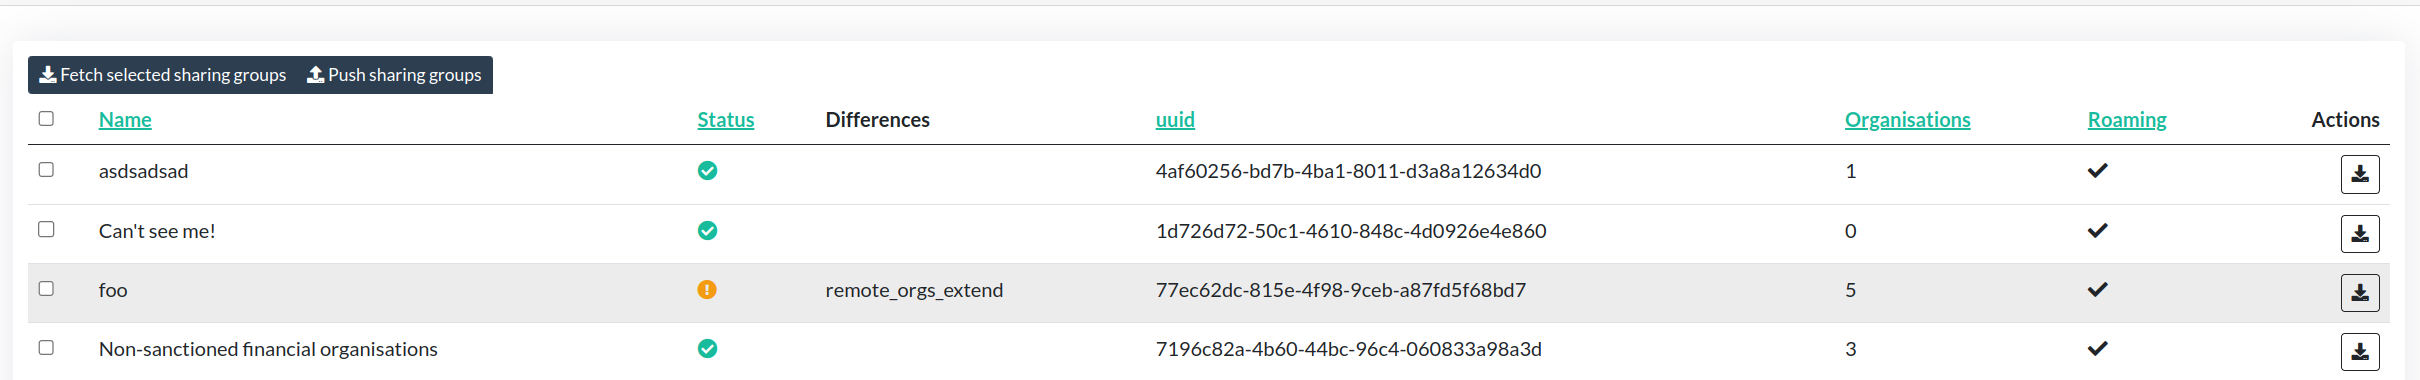
\includegraphics[width=1.0\linewidth]{pictures/orchestration2.png}
    \end{center}
\end{frame}

\begin{frame}
\frametitle{Push rules}
    \begin{center}
        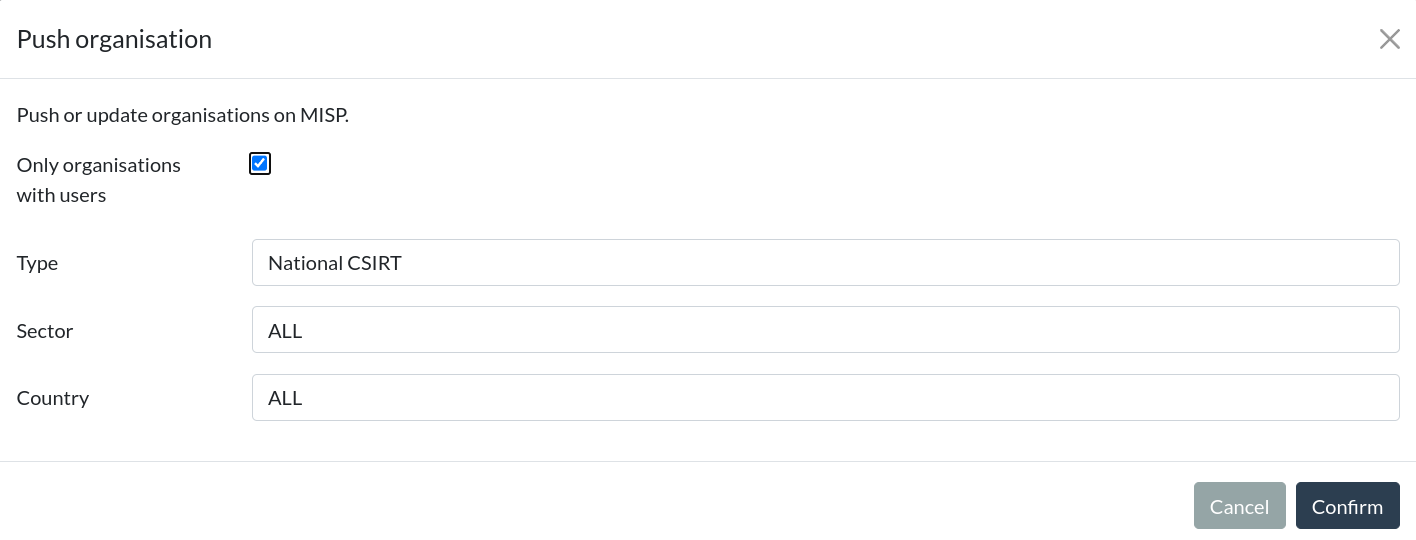
\includegraphics[width=1.0\linewidth]{pictures/orchestration3.png}
    \end{center}
\end{frame}

\begin{frame}
\frametitle{Quality of life improvements}
    \begin{itemize}
        \item Meta-template {\bf version migrations} rework
        \begin{itemize}
 	       \item Various supported strategies (update, delete)
        \end{itemize}
        \item New community management settings
        \item {\bf CLI tools} for enrollment
        \item UI rework to streamline user interactions
    \end{itemize}
\end{frame}

\begin{frame}
\frametitle{Quality of life improvements}
    \begin{itemize}
        \item {\bf Download filtered results}
        \item Export as {\bf CSV}
        \item Includes all custom meta-fields
    \end{itemize}
\end{frame}

\begin{frame}
\frametitle{Quality of life improvements}
    \begin{itemize}
        \item {\bf Search and filter based on custom fields}
        \item Define rules on what to display in terms of custom fields by default
        \item Search on related data
        \item Modify and {\bf extend roles} with metafields
    \end{itemize}
\end{frame}

\begin{frame}
\frametitle{Sharing group rework}
    \begin{itemize}
        \item Match what MISP does
        \item Sharing group extenders
        \item {\bf Sync sharing groups to/from MISP}
    \end{itemize}
\end{frame}

\begin{frame}
\frametitle{Cake-fuzzer}
    \begin{itemize}
        \item Developped by {\bf Zigrin security}, run by NCIA alumn {\bf Dawid Czarnecki}
        \item Funded by the {\bf Luxembourg Armed Forces}
        \item Full blown {\bf fuzzing framework targeting MISP and Cerebrate}
        \item Long list of {\bf high severity CVEs} discovered
        \item Constant development, open source
        \item Will become part of our release CI pipeline
        \item \url{https://github.com/Zigrin-Security/CakeFuzzer}
    \end{itemize}
\end{frame}



\section{What we're working on}

\begin{frame}
\frametitle{Issues we're trying to solve as of late for ourselves}
    \begin{itemize}
        \item {\bf Contact management} across large interconnected networks
        \item {\bf Constituency} information
         \begin{itemize}
            \item Geographic \& sectorial
            \item But also technical: CIDR blocks \& AS Numbers
        \end{itemize}
	\item Managing our MISP fleets for various use-cases
	\item {\bf Distribution list} management
	\item MISP cryptographic signing {\bf PKI} management
	 \begin{itemize}
            \item MISP's protected event feature
            \item Future: Protected Sharing groups? 
        \end{itemize}
        \item Creating data buckets in MISP for better retrieval
        \item Sub-group self management
    \end{itemize}
\end{frame}

\begin{frame}
\frametitle{A bit about our internal topology}
  \begin{center}
    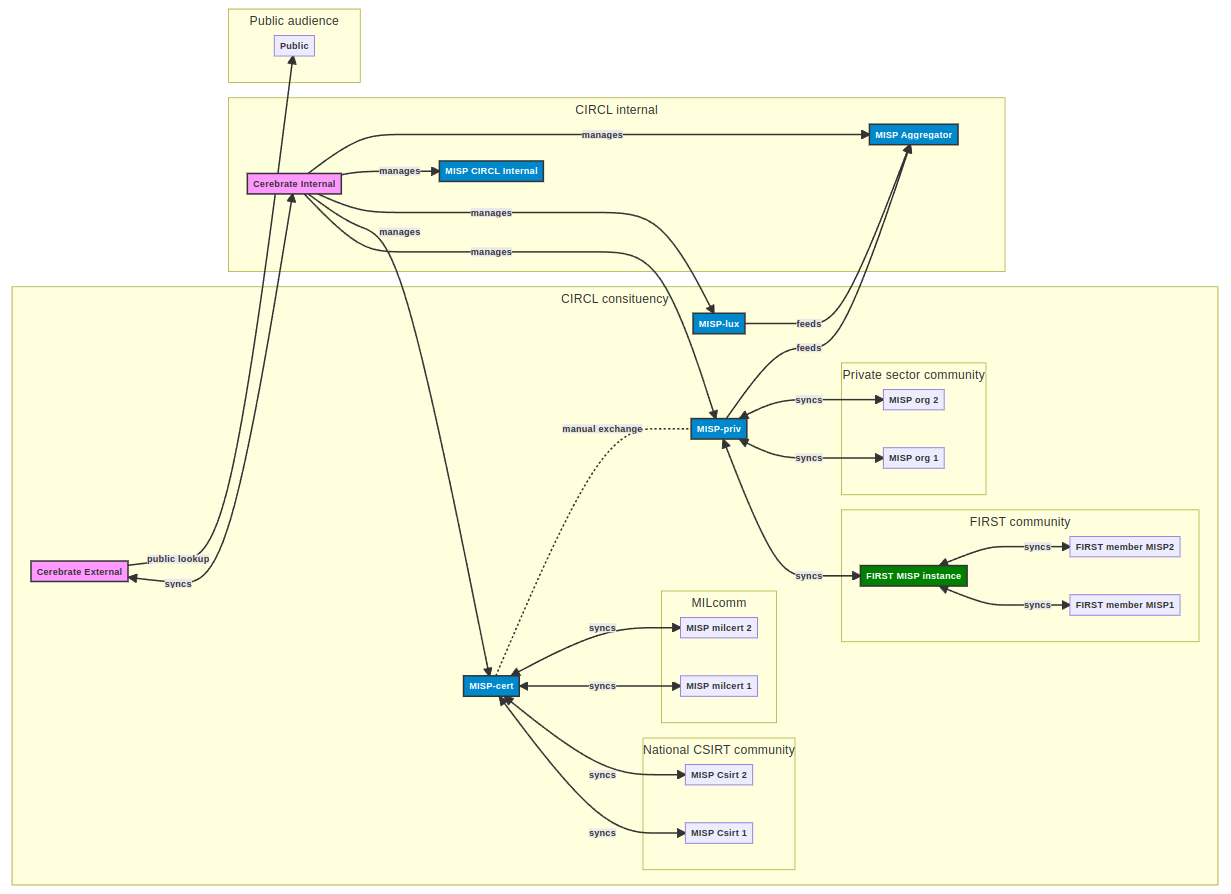
\includegraphics[width=1\linewidth]{pictures/our_topology.png}
  \end{center}
\end{frame}


\begin{frame}
\frametitle{Deployment}
    \begin{itemize}
        \item \textbf{Deploying} the topology above
        \item Standing up a {\bf NATO community Cerebrate} instance
            \begin{itemize}
            	\item Details to be finalised, hosted at CIRCL
            	\item Based on previous discussions at MUG and steering board
            \end{itemize}
        \item \textbf{Deploying} an Open lookup Cerebrate 
        \item Supporting the finalisation of the CNW deployment
    \end{itemize}
\end{frame}

\begin{frame}
\frametitle{Development}
    \begin{itemize}
        \item Further MISP integrations
        \item Integration with other tools
        \item Community centric PKI
        \begin{itemize}
            \item Protected mode support
            \item General data signing support for MISP
        \end{itemize}
        \item Mailing group management
    \end{itemize}
\end{frame}


